\documentclass{article}
\usepackage{fasy-hw}

\author{Joshua Harthan}
\problem{1}
\begin{document}
8.5 Question 14
\item[]Prove that for all positive integers $a$ and $b$, $a | b$ if, and only if, lcm($a,b) = b$.
\item[]Case 1: If $a | b$, then lcm$(a,b) = b$
\item[]From the definition of the least common multiple of two nonzero integers $a$ and $b$, there is a positive integer $c$ such that $a|c$ and $b|c$, where $c$ is the lcm(a,b). If we are to sub in the value of $b$ for $c$, we get $a|b$ and $b|b$, which is true as $b$ is divisible by itself and $a$ is divisible by $b$, with lcm($a,b$) = $b$. So, from the definition of the least common multiple, if $a|b$ and $b|b$, the lcm($a,b$) = $b$. Therefore, if $a|b$, then lcm$(a,b) = b$.

\item[]Case 2: If lcm$(a,b) = b$, then $a|b$
\item[]From the definition of the least common multiple of two nonzero integers $a$ and $b$, is the positive integer $c$ such that 
that $a|c$ and $b|c$. So if $c$ is the lcm($a,b$), if we are to sub in the value of $b$ for $c$ we get lcm($a,b)$ = $b$, where $a|b$ and $b|b$. Therefore, if lcm$(a,b) = b$, then $a|b$

Therefore, for all positive integers $a$ and $b$, $a | b$ if, and only if, lcm($a,b) = b$.

\problem{2}
\collab{none}
\clearpage
\header
8.5 Question 30
\item[]Solve the congruence of $2184 \; \equiv \; 5481$ (mod 286).
\item[]From question 28, it is given that for all integers $a, \: c,$ and $n$ with $n > 1$, if gcd($a,n$) = $d$ and $d$ divides $c$, then the congruence $ax \: \equiv \: c$ (mod $n$) has a solution. So from this, we can say that gcd(2184,286) = 26 since 2184 = 26 $\cdot$ 84 and 286 = 26 $\cdot$ 11; no integer larger than 26 divides both 2184 and 286. However, 5481 is not divisible by 26, i.e. $26 \nmid 5481$. Therefore, there does not exist a solution to the congruence equation $2184 \; \equiv \; 5481$ (mod 286).


\problem{3}
\collab{none}
\clearpage
\header
3.1 What is gcd(91,42)?
\item[] 91 = 7 $ \cdot $ 13 and 42 = 7 $ \cdot $ 6. So $7 \: | \: 91$ and $7 \: | \: 42$, and no integer larger than 7 divides both 91 and 42. Therefore, gcd(91,42) = 7.
\item[]3.2 What is lcm(37,15)? 
\item[] 555 = 37 $ \cdot $ 15 and 555 = 15 $ \cdot $ 37. So $37 \: | \: 555$ and $15 \: | \: 555$, and no integer that is less than 555 is divisible by both 15 and 37. Therefore, lcm(37,15) = 555. 


\problem{4}
\collab{none}
\clearpage
\header
What are the additive and multiplicative inverses of the elements of $Z_{9}$ and $Z_{11}$ (where the inverses exist)? 
\item Show the addition and multiplication tables for each.
\item[]\begin{center}
 \begin{tabular}{||c c c c c c c c c c||} 
 \hline
 ($\mathbb{Z}_{9}, +_{9})$ & 0 & 1 & 2 & 3 & 4 & 5 & 6 & 7 & 8 \\ [0.5ex] 
 \hline\hline
 0 & 0 & 1 & 2 & 3 & 4 & 5 & 6 & 7 & 8 \\
 \hline
 1 & 1 & 2 & 3 & 4 & 5 & 6 & 7 & 8 & 0 \\ 
 \hline
 2 & 2 & 3 & 4 & 5 & 6 & 7 & 8 & 0 & 1 \\
 \hline
 3 & 3 & 4 & 5 & 6 & 7 & 8 & 0 & 1 & 2 \\
 \hline
 4 & 4 & 5 & 6 & 7 & 8 & 0 & 1 & 2 & 3 \\
 \hline
 5 & 5 & 6 & 7 & 8 & 0 & 1 & 2 & 3 & 4 \\ 
 \hline
 6 & 6 & 7 & 8 & 0 & 1 & 2 & 3 & 4 & 5\\
 \hline
 7 & 7 & 8 & 0 & 1 & 2 & 3 & 4 & 5 & 6\\
 \hline
 8 & 8 & 0 & 1 & 2 & 3 & 4 & 5 & 6 & 7\\ [0.5ex] 
 \hline 
\end{tabular}
\end{center} 


\item[]\begin{center}
 \begin{tabular}{||c c c c c c c c c c||} 
 \hline
 ($\mathbb{Z}_{9}, \times_{9})$ & 0 & 1 & 2 & 3 & 4 & 5 & 6 & 7 & 8 \\
 \hline\hline
 0 & 0 & 0 & 0 & 0 & 0 & 0 & 0 & 0 & 0 \\
 \hline
 1 & 0 & 1 & 2 & 3 & 4 & 5 & 6 & 7 & 8 \\ 
 \hline
 2 & 0 & 2 & 4 & 6 & 8 & 1 & 3 & 5 & 7 \\
 \hline
 3 & 0 & 3 & 6 & 0 & 3 & 6 & 0 & 3 & 6 \\
 \hline
 4 & 0 & 4 & 8 & 3 & 7 & 2 & 6 & 1 & 5 \\
 \hline
 5 & 0 & 5 & 1 & 6 & 2 & 7 & 3 & 8 & 4 \\ 
 \hline
 6 & 0 & 6 & 3 & 0 & 6 & 3 & 0 & 6 & 3\\
 \hline
 7 & 0 & 7 & 5 & 3 & 1 & 8 & 6 & 4 & 2\\
 \hline
 8 & 0 & 8 & 7 & 6 & 5 & 4 & 3 & 2 & 1\\ 
 \hline 
\end{tabular}
\end{center}

\item[] Additive Inverses: -0 = 0, -1 = 8, -2 = 7, -3 = 6, -4 = 5, -5 = 4, -6 = 3, -7 = 2, -8 = 1
\item[] Multiplicative Inverses: $1^{-1} = 1$, $2^{-1} = 5$, $3^{-1} =$ DNE, $4^{-1} = 7$, $5^{-1} = 2$, $6^{-1} =$ DNE, $7 ^{-1} = 4$, $8^{-1} = 8$

\problem{4(cont.)}
\collab{none}
\clearpage
\header
\item[]\begin{center}
 \begin{tabular}{||c c c c c c c c c c c c ||} 
 \hline
 ($\mathbb{Z}_{11}, +_{11})$ & 0 & 1 & 2 & 3 & 4 & 5 & 6 & 7 & 8 & 9 & 10 \\ [0.5ex] 
 \hline\hline
 0 & 0 & 1 & 2 & 3 & 4 & 5 & 6 & 7 & 8 & 9 & 10\\
 \hline
 1 & 1 & 2 & 3 & 4 & 5 & 6 & 7 & 8 & 9 & 10 & 0 \\ 
 \hline
 2 & 2 & 3 & 4 & 5 & 6 & 7 & 8 & 9 & 10 & 0 & 1 \\
 \hline
 3 & 3 & 4 & 5 & 6 & 7 & 8 & 9 & 10 & 0 & 1 & 2 \\
 \hline
 4 & 4 & 5 & 6 & 7 & 8 & 9 & 10 & 0 & 1 & 2 & 3 \\
 \hline
 5 & 5 & 6 & 7 & 8 & 9 & 10 & 0 & 1 & 2 & 3 & 4 \\ 
 \hline
 6 & 6 & 7 & 8 & 9 & 10 & 0 & 1 & 2 & 3 & 4 & 5 \\
 \hline
 7 & 7 & 8 & 9 & 10 & 0 & 1 & 2 & 3 & 3 & 5 & 6 \\
 \hline
 8 & 8 & 9 & 10 & 0 & 1 & 2 & 3 & 4 & 5 & 6 & 7 \\ 
 \hline 
 9 & 9 & 10 & 0 & 1 & 2 & 3 & 4 & 5 & 6 & 7 & 8 \\
 \hline 
 10 & 10 & 0 & 1 & 2 & 3 & 4 & 5 & 6 & 7 & 8 & 9 \\
 \hline
\end{tabular}
\end{center} 

\item[]\begin{center}
 \begin{tabular}{||c c c c c c c c c c c c ||} 
 \hline
 ($\mathbb{Z}_{11}, \times_{11})$ & 0 & 1 & 2 & 3 & 4 & 5 & 6 & 7 & 8  & 9 & 10 \\ [0.5ex] 
 \hline\hline
 0 & 0 & 0 & 0 & 0 & 0 & 0 & 0 & 0 & 0  & 0 & 0 \\
 \hline
 1 & 0 & 1 & 2 & 3 & 4 & 5 & 6 & 7 & 8 & 9 & 10 \\ 
 \hline
 2 & 0 & 2 & 4 & 6 & 8 & 10 & 1 & 3 & 5 & 7 & 9 \\
 \hline
 3 & 0 & 3 & 6 & 9 & 1 & 4 & 7 & 10 & 2 & 5 & 8 \\
 \hline
 4 & 0 & 4 & 8 & 1 & 5 & 9 & 2 & 6 & 10 & 3 & 7 \\
 \hline
 5 & 0 & 5 & 10 & 4 & 9 & 3 & 8 & 2 & 7 & 1 & 6 \\ 
 \hline
 6 & 0 & 6 & 1 & 7 & 2 & 8 & 3 & 9 & 4 & 10 & 5 \\
 \hline
 7 & 0 & 7 & 3 & 10 & 6 & 2 & 9 & 5 & 1 & 8 & 4 \\
 \hline
 8 & 0 & 8 & 5 & 2 & 10 & 7 & 4 & 1 & 9 & 6 & 3 \\ 
 \hline 
 9 & 0 & 9 & 7 & 5 & 3 & 1 & 10 & 8 & 6 & 4 & 2 \\
 \hline 
 10 & 0 & 10 & 9 & 8 & 7 & 6 & 5 & 4 & 3 & 2 & 1 \\
 \hline
\end{tabular}
\end{center}

\item[] Additive Inverses:  -0 = 0, -1 = 10, -2 = 9, -3 = 8, -4 = 7, -5 = 6, -6 = 5, -7 = 4, -8 = 3 , -9 = 2, -10 = 1
\item[] Multiplicative Inverses: $1^{-1} = 1$, $2^{-1} = 6$, $3^{-1} = 4$, $4^{-1} = 3$, $5^{-1} = 9$, $6^{-1} = 2$, $7 ^{-1} = 8$, $8^{-1} = 7$, $9^{-1} = 5$, $10^{-1} = 10$


\problem{5}
\collab{none}
\clearpage
\header
For the following, draw a map (with coloring or colorings) that has at least 5 faces and satisfies the following:
\item[]5.1 Has a two-coloring. Show the coloring.
\begin{figure}[h!]
  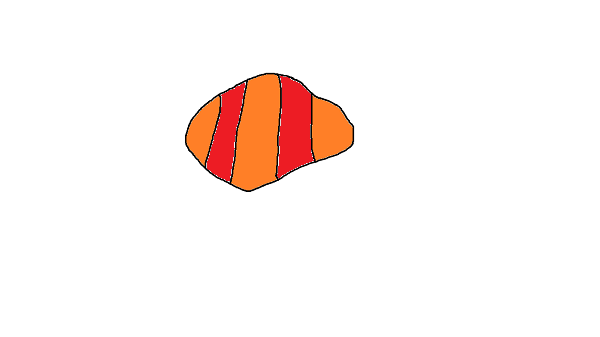
\includegraphics[width=\linewidth]{Untitled.png}
  \caption{Map with two-coloring}
  \label{fig:map1}
\end{figure}

\problem{5 (cont.)}
\collab{none}
\clearpage
\header
\item[]5.2 Has a three-coloring, but not a two-coloring.
\begin{figure}[h!]
  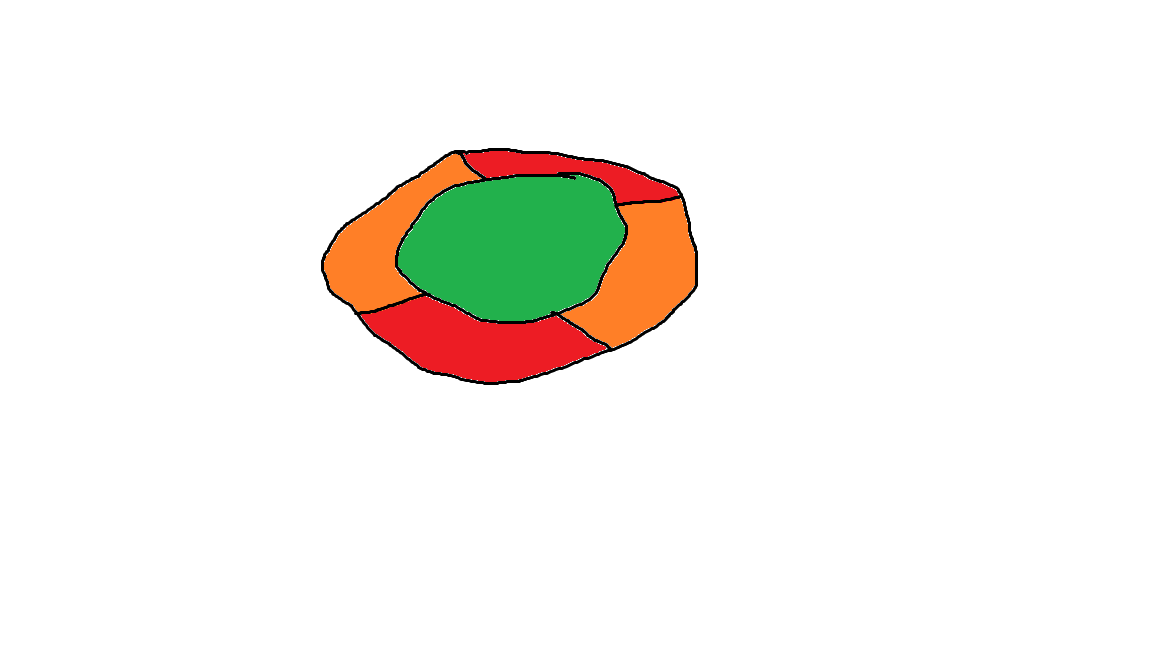
\includegraphics[width=\linewidth]{Untitled1.png}
  \caption{Map with three-coloring}
  \label{fig:map1}
\end{figure}

\problem{5 (cont.)}
\collab{none}
\clearpage
\header
\item[]5.3 Has a four-coloring, but not a three-coloring.
\begin{figure}[h!]
  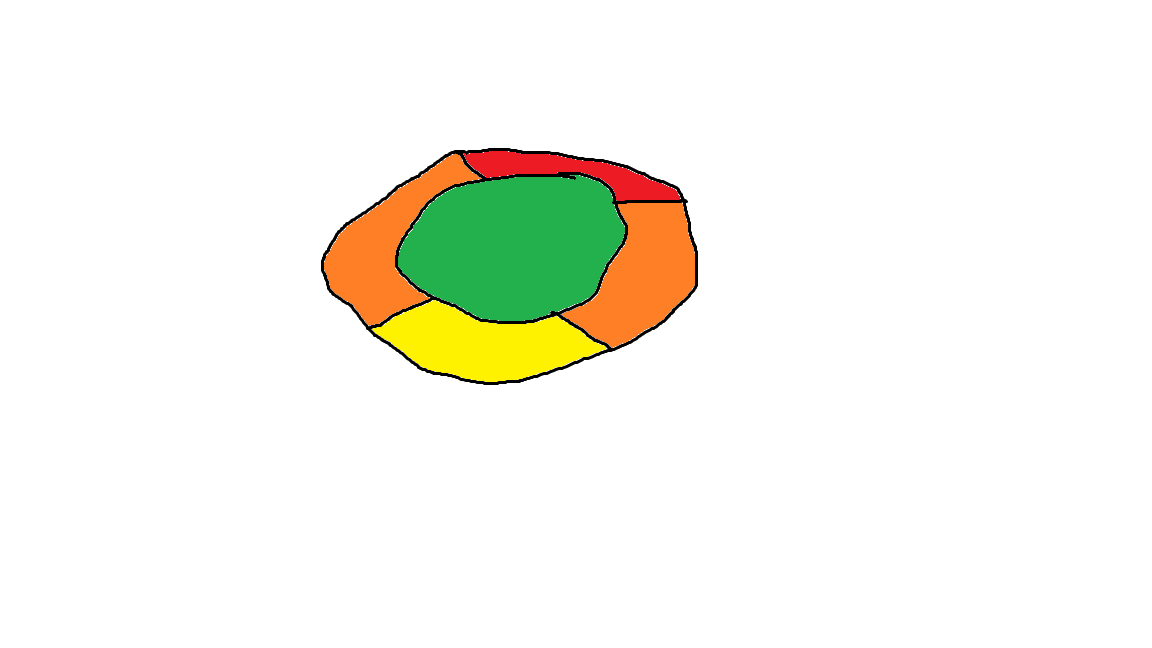
\includegraphics[width=\linewidth]{Untitled2.png}
  \caption{Map with four-coloring}
  \label{fig:map1}
\end{figure}

\problem{5(cont.)}
\collab{none}
\clearpage
\header
\item[]5.4 Has two different colorings (that are not simply a relabeling of the same coloring).
\begin{figure}[h!]
  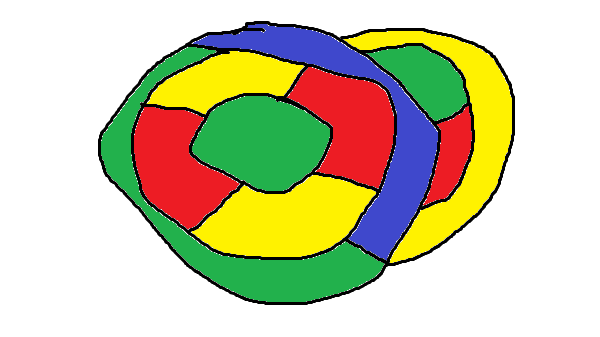
\includegraphics[width=\linewidth]{Untitled3.png}
  \caption{Map with two different colorings}
  \label{fig:map1}
\end{figure}

\problem{6}
\collab{none}
\clearpage
\header
\item[] Frances Allen is an American computer scientist who worked in the field of optimizing computer compilers. Optimizing a compiler in computer science is the act of minimizing or maximizing certain attributes within a program, such as minimizing the time or amount of memory that a program uses to execute. Allen was known for creating different algorithms and implementations that allowed for more optimal programming, and worked on the development of different programming languages and computers while she worked for IBM. Allen is important to the field of computer science in that she helped to develop more optimal ways in which programs are executed, something that is always needed as time goes on. Without people like Allen laying down the groundwork for compiler optimization, we would not be able to build on her work and further optimize programs.

\item[]\url{https://en.wikipedia.org/wiki/Frances_E._Allen}
\item[]\url{https://en.wikipedia.org/wiki/Optimizing_compiler}

\end{document}